\section{Sparse LU Decomposition}

The matrix multiplication equation \(A = LU\), with L unit lower triangular U upper
triangular, and  can be rewritten to give the expressions for L and U as follows:
\begin{subequations}
    \centering
    \begin{align}
        U_{(i,j)} & = A_{(i,j)} - \sum\limits_{k = 1}^{i-1} L_{(i,k)}U_{(k,j)} \\
        L_{(i,j)} & = \frac{A_{(i,j)} - \sum\limits_{k = 1}^{j-1} L_{(i,k)}U_{(k,j)}}{U_{(j,j)}}
    \end{align}
    \label{eqn:LUD:LUequation}
\end{subequations}

The same Gaussian elimination can be used in a factorization of sparse matrices.
Since the column vectors are sparse, some of the inner products reduces to zero and hence
can be excluded for the update rule. However, since it may be
necessary to pivot based on previously updated elements, a sparse Gaussian elimination
algorithm cannot know the exact nonzero structure of these vectors in advance of all
numerical computation. \\
Direct methods of sparse LU decomposition are widely divided into three categories.
Left-looking, Right-Looking and Crout \cite{crout}. These methods are characterized
by the factor update (Multiply and Accumulate) and normalization (Division) rules.
\\
\\
\textbf{Left-Looking}
\\
Left-looking algorithms factorizes the matrix in column-by-column manner. Factors
of current column are updated using the previously computed columns with
equation \(A_{(i,j)} = A_{(i,j)} - L_{(i,k)} \times U_{(k,j)} \), where 
\(k = [1, \cdots, min(i,j)]\). Updated factors are then normalized with the pivot value.
\\
\\
\textbf{Right-Looking} 
\\
The Right looking algorithm first factorizes a column from the lower triangular part 
of a matrix, then uses the resulting non-zero elements of that column to update 
the affected components in the rest of the matrix by using the equation
\(A_{(i,k)} = A_{(i,k)} - L_{(i,j)} \times U_{(j,k)} \), where \(k = [j+1, \cdots, N]\),
j is the index of current factored column, and N is the column dimension of matrix A
\\
\\
\textbf{Crout}
\\
Similar to the Left-looking algorithm, the Crout method performs updates with 
previously factored elements before normalizing a given vector. The difference 
is that the Crout method operates both on columns and rows, while the Left-looking
algorithm only operates on columns. (See figure \ref{fig:LUD:algos})

\begin{figure}[H]
    \centering
    \begin{subfigure}[b]{0.33\textwidth}
        \includegraphics[width = 0.95\linewidth]{./Theory/leftLooking.JPG}
        \caption{Left-Looking}
        \label{fig:LUD:leftLooking}
    \end{subfigure}%
    \begin{subfigure}[b]{0.33\textwidth}
        \includegraphics[width = 0.95\linewidth]{./Theory/rightLooking.JPG}
        \caption{Right-Looking}
        \label{fig:LUD:rightLooking}
    \end{subfigure}%
    \begin{subfigure}[b]{0.33\textwidth}
        \includegraphics[width = 0.95\linewidth]{./Theory/crout.JPG}
        \caption{Crout}
        \label{fig:LUD:crout}
    \end{subfigure}
    \caption{Algorithms for Sparse LU Decomposition}
    \label{fig:LUD:algos}
\end{figure}

\subsection{AMD Ordering}
An Approximate Minimum Degree ordering algorithm (AMD) for
pre-ordering a symmetric sparse matrix prior to numerical factorization
is presented. The Cholesky factorization of ordered symmetric matrices tends to be 
sparser than that of the original ones. This method can be extended to asymmetric matrix, say $A$, by applying 
the AMD on $A + A'$. Pre-ordering the matrices reduces the number of fill-ins in the 
factors and hence reduces the number of required floating point operations dramatically.

\begin{figure}
    \centering
    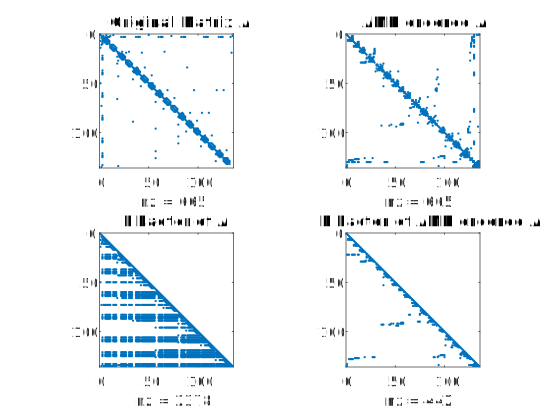
\includegraphics[width = 0.9\linewidth]{./Theory/amd.pdf}
    \caption{Effect of AMD ordering on the factorization of the $135\times135$ Matrix}
    \label{fig:AMD:AMDeffect}
\end{figure}

The figure \ref{fig:AMD:AMDeffect} demonstrates the effect of AMD ordering on the 
\textit{Rajat11}, a matrix of order $135\times135$. As reduction in the \textit{NNZ} 
increases significantly as the order increases. \\
A linear problem $Ax = b$ can be solved by solving the reordered problem where $P$ is the 
AMD permutation matrix.

\begin{equation}
    \centering
    (P^TAP)(P^Tx) = P^Tb
    \label{eqn:AMD:ModifiedLinear}
\end{equation}